\documentclass{article}

\usepackage[utf8]{inputenc}
\usepackage[english, russian]{babel}
\usepackage{graphicx}

\begin{document}
	\paragraph{Геометрия, неравенства, задача 7?}\hspace{\fill}
	\newline
	Докажем, что ГМТ X, таких, что $AX + BX = CX + DX$ - это серединный перпендикуляр к стороне АС(он же серединный перпендикуляр к стороне BD). Обозначим его точки пересечения со сторонами прямоугольника за К и N. 
	Тогда для любой M1, которая принадлежит прямой KN, справедливо \newline
	$AM1 = \sqrt{AK^2 + KM1^2}, CM1 = \sqrt{KM1^2 + KC^2}, AM1 = CM1, $ тк $  KC = AK$
	\newline
	$BM1 = \sqrt{BN^2 + NM1^2}, DM1 = \sqrt{NM1^2 + Dn^2}, BM1 = DM1, $ тк $  NB = ND$	
	\newline
	Тогда AM1 + BM1 = CM1 + DM1.
	\newline
	Докажем, что не существует таких точек, которые не принадлежат прямой KN и принадлежат нашему ГМТ.
	\newline
	Пусть есть точка M2, такая, что AM2 + BM2 = CM2 + DM2. Проведем через M2 прямую, параллельную KN, назовем точки пересечения с прямоугольником K' и N'. Для определенности будем считать, что мы взяли М2 в той полуплоскости относительно KN, в которой AK' < K'C(и соответственно BN' < N'D)
	\newline
	Посчитаем сумму расстояний 
	\newline
	$AM2 = \sqrt{AK'^2 + M2K'^2}, CM2 = \sqrt{CK'^2 + M2K'^2}. $ тк $CK' > AK', $ то $AM2 < CM2$
	\newline	
	$BM2 = \sqrt{BN'^2 + M2N'^2}, DM2 = \sqrt{DN'^2 + M2N'^2}. $ тк $DN' > BN', $ то $BM2 < DM2$
	\newline
	Отсюда $AM2 + BM2 < CM2 + DM2$
	\newline
	Аналогичными рассуждениями, взяв точку M3 в противоположной полуплоскости относительно KN, получим $AM3 + BM3 > CM3 + DM3$
	Тогда точки M2 и M3 не принадлежат ГМТ.
	\newline
	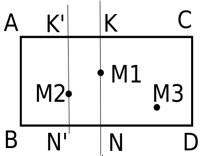
\includegraphics{rect1.png}
	\newline
	\textbf{Ответ} - серединный перпендикуляр к стороне АС
\end{document}